\documentclass[12pt]{article}
%\usepackage{mathptmx}
\usepackage{graphicx}
\usepackage{amsmath}
\usepackage{amssymb}
\author{John Finn}
\date{April 22, 2004}
\title{Make Circle}
\begin{document}
\maketitle
\tableofcontents
\section{Opening Comments}

This gives the programming answer to a question posed by Robert Heller:

\begin{itemize}
\item Given the radius and two points on a circle, can we determine the circle?
\end{itemize}

A moment's reflection reveals that to determine the circle here means to find the center.
  
The answer is ``almost'', which is not hard to see if we begin by sketching the desired
circle, calling its center M.  I think it's best to make the circle a dotted line, since
we're going to pretend we don't know just where it is.  We sketch the points A and C 
somewhere along its circumference, making them boldface, say, to indicate that we do 
know just where they are.  The center M we make faint, since we start out not knowing
where it is.  Since do know the radius r, we begin by setting a compass to that size.

Now we use the compass to draw two r-sized circles, whose centers are A and C.  If
you take the time to actually make the sketch, or if you have a good visual imagination, 
you'll see that these two circles intersect in two points, one of which is M ---well, 
that is, unless A and C happen to be exactly the endpoints of a diameter, in 
which case the two circles intersect at just the single point M.

But in the generic case, if A and C are just any old points on the unknown circle, 
then the unknown center M is one of the two points of intersection of the two circles we
construct.  This is why the answer is ``almost'';  without further information, we have
two possible answers.  For the further information, Heller suggests that we stipulate 
that C lie counterclockwise from A on the circle, meaning that in drawing the shortest 
arc from A to C our pencil moves counterclockwise.  (This is again ambiguous in the case
that A and C are diametrically opposite, but again in that special case we only have a 
single intersection, and so don't need to know the relative positions of A and C).

Notice also that while we {\em could}, for given points A and C, give values for r for 
which no solution exists, it's easy to recognize these impossible cases; they're exactly
the ones where r is less than half the distance between A and C.

This program lets the user use the mouse to
\begin{itemize}
\item pick points A and C, and then 
\item specify a value for r by picking a point whose distance from A will be taken as r.
\end{itemize}
The program will then draw the two intersecting circles with centers at A and C, figure
out algebraically their two points of intersection, and pick as M the one that gives A
and C the right orientation.  It will then show which is C, and plot the circle we're
trying to find.

An explanation of the algebra  ---which amounts to finding the two solutions to two
quadratic equations in two unknowns--- is appended at the bottom of the program itself;
these opening remarks are already long enough! 

\section{Detailed Explaination}

\subsection{Problem}

Suppose we have points $\vec{a} = (a,b)$ and $\vec{c} =
(c,d)$ in the plane, and know they lie on a circle whose radius $r$ we
also know.  Find the circle.

\subsection{Solution}

First, since we know $r$, to determine the circle it is enough to find
its center, $\vec{m} = (m,n)$. To do so, construct a circle of
radius $r$ about each of $\vec{a}$ and $\vec{c}$:


\includegraphics{FinnFigure1}

Now the two (generically) points of intersection of these two circles
are {\em both} centers of circles radius $r$ that contain
$\vec{a}$ and $\vec{c}$. For a unique solution, we
need to add a condition to those given, so we specify that the
orientation of $\vec{a}$ and $\vec{c}$ by
requiring that $\vec{c}$ be counterclockwise from
$\vec{a}$ on the circle--meaning that the {\em shorter} of
the 2 arcs joining $\vec{a}$ to $\vec{c}$ is in
the counterclockwise (or mathematically positive) direction.

\begin{tabular}[c]{cc}
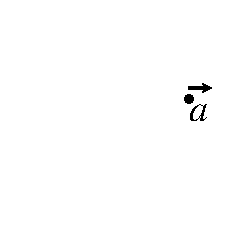
\includegraphics{FinnFigure2a} & 
\includegraphics{FinnFigure2b} \\
$\overset{\curvearrowright}{\vec{a}\vec{c}}$ counterclockwise &
$\overset{\curvearrowright}{\vec{a}\vec{c}}$ clockwise \\
\end{tabular}

To determine $\vec{m}$, think of it for the nonce as the unknown $\vec{x}
= (x,y)$. We then have 2 quadratic equations in x and y:


\begin{equation}
{(x-a)}^2 + {(y-b)}^2 = r^2
\label{e1}
\end{equation}
and
\begin{equation}
{(x-c)}^2 + {(y-d)}^2 = r^2
\label{e2}
\end{equation}

%(\ref{e1}) means: ``$(x,y)$ is on the circle of radius $r$ about
%$(a,b)$'' or ``the distance (squared) from $(x,y)$ to $(a,b)$ is $r$
%(squared)''.

expanding these out, and substracting (\ref{e1}) from
(\ref{e2}) we get (after gathering terms and factoring):

\begin{equation}
\frac{\begin{aligned}
	x^2-2cx+c^2+y^2-2dy+d^2&=r^2\\
      -(x^2-2ax+a^2+y^2-2by+b^2&=r^2)\\
      \end{aligned}}{2(a-c)x+2(b-d)y=(a^2+b^2)-(c^2+d^2)}
\end{equation}

Now this may look complicated, but it's just

\begin{equation}
Jx+Gy=T
\label{e4}
\end{equation}

and (\ref{e4}) is linear in $x$ and $y$, so trivial to solved for
$y$ in terms of $x$:

\begin{equation}
y = \frac{T-Jx}{G}
\label{eq5}
\end{equation}

Doing this eliminates $y$ (at least for the nonce) and gives a quadratic
equation in just the single variable $x$. That is, if we plug in
$\frac{T-Jx}{G}$ for $y$, in either (\ref{e1}) or (\ref{e2}), we get a
quadratic in $x$--which we can solve by plugging in its coefficients
into the quadratic formula.  The quadratic will give {\em 2} values for
$x$, one for each of the two points $m_1$ and $m_2$ shown earlier.

So we take (\ref{e1}) plug in $y = \frac{T-Jx}{G}$:

\begin{equation}
{(x-a)}^2+{\left(\frac{T-Jx}{G}-b\right)}^2=r^2
\label{eq6}
\end{equation}

and now expand this out enough to identify $x^2$, $x$, and constant
terms

\begin{gather}
x^2-2ax+a^2+{\left(\frac{T-Jx}{G}\right)}^2
-2\left(\frac{T-Jx}{G}\right)b+b^2=r^2\\
x^2-2ax+a^2+\frac{T^2-2JTx+J^2x^2}{G^2}
-2\left(\frac{T-Jx}{G}\right)b+b^2=r^2
\end{gather}

so we have

\begin{alignat}{3}
\left(1+\frac{J^2}{G^2}\right)&x^2 & 
	+\left(-2a-\frac{2JT}{G^2}+\frac{2bJ}{G}\right)&x &
	+\left((a^2+b^2)+\frac{T^2}{G^2}-\frac{2bJ}{G}-r^2\right)& = 0\\
u&x^2 &+ v&x &+ w& = 0
\end{alignat}


Now we {\em could} express each of these coeff's in terms of $a,b,c,d$,
and grind away to try to simplfy them, but if we just want them for a
computer program, there's no need to--which is good, because they {\em
don't} simplify a great deal.

Our {\rm two} answers, then are

\begin{equation}
x = \frac{-v\pm\sqrt{v^2-4uw}}{2u},
\end{equation}
and
\begin{equation}
y = \frac{T-Jx}{G}
\end{equation}

with each of the $x$'s plugged in.

Finally, to pick the right $(x,y)$ for $(m,n)$--that is, to deal with
the orientation, we note that the $\vec{c}$ counterclockwise from
$\vec{a}$ means exactly that the angle from $\vec{a}$ to $\vec{c}$ be
between $0$ and ${180}^\circ$--well, modulo $2\pi$.  But this is also true
if the and only if the sine of this angle is positive.  So we see which
of

\begin{equation}
\sin(\arctan(\vec{a}-\vec{m_1},\vec{c}-\vec{m_1}))
\end{equation}
and
\begin{equation}
\sin(\arctan(\vec{a}-\vec{m_2},\vec{c}-\vec{m_2}))
\end{equation}

is positive, and we're done.


\end{document}

